\documentclass[14pt]{extarticle}
\usepackage{fontspec}
\usepackage[ukrainian]{babel}
\usepackage[contents=TODO, color=gray, pages=some]{background}
\usepackage[a4paper, left=20mm, top=20mm, right=10mm, bottom=20mm]{geometry}
\usepackage{indentfirst}
\usepackage{titlesec}
\usepackage{stringstrings}
\usepackage{fancyhdr}
\usepackage{enumitem}
\usepackage{tabularx}
\usepackage[hidelinks]{hyperref}
\usepackage{textcase}
\usepackage{url}
\usepackage{csquotes}
\usepackage[style=numeric, sorting=none]{biblatex}
\usepackage{graphicx}
\usepackage{float}
\usepackage{caption}
\usepackage{listings}

\lstnewenvironment{mycode}[1][]{
  \lstset{
    basicstyle=\small\ttfamily,
    captionpos=b,
    #1
  }
}{}

\DeclareCaptionLabelFormat{dstuFigLabel}{Рисунок #2}
\DeclareCaptionLabelSeparator{abobasep}{ --- }
\captionsetup[figure]{labelformat = dstuFigLabel
                     ,labelsep    = abobasep
                     }

\addbibresource{zapiska.bib}

% TODO: make section uppercase in embedded links

% Uppercase sections in ToC
\makeatletter
\let\oldcontentsline\contentsline
\def\contentsline#1#2{%
  \expandafter\ifx\csname l@#1\endcsname\l@section
    \expandafter\@firstoftwo
  \else
    \expandafter\@secondoftwo
  \fi
  {%
    \oldcontentsline{#1}{\MakeTextUppercase{#2}}%
  }{%
    \oldcontentsline{#1}{#2}%
  }%
}
\makeatother

\hypersetup{linktoc=all}

\pagestyle{fancy}
\fancyhf{}
\fancyhead[R]{\thepage}
\renewcommand{\headrule}{}
\setlength{\headheight}{17pt}

\setmainfont{Times New Roman}
\linespread{1.5}
\setlength{\parindent}{16mm}

\titleformat{\section}
  { \filcenter % center
    \fontsize{14pt}{14pt}
    \bfseries % semi bold
    \MakeUppercase
  }
  {\thesection~}
  {0pt}
  {}
\titlespacing*{\section}{0pt}{12pt}{6pt}

\titleformat{\subsection}
  { \fontsize{14pt}{14pt}
  }
  % TODO: sentence case
  {\thesubsection~}
  {0pt}
  {}
\titlespacing*{\subsection}{0pt}{6pt}{0pt}

\titleformat{\subsubsection}
  { \fontsize{14pt}{14pt}
  }
  % TODO: sentence case
  {\thesubsubsection~}
  {0pt}
  {}
\titlespacing*{\subsubsection}{0pt}{6pt}{0pt}

% all sections will start at new page
\let\oldsection\section
\renewcommand{\section}{\clearpage\oldsection}

\newcommand{\unnumberedSection}[1]{%
  \section*{#1}%
  \phantomsection
  \addcontentsline{toc}{section}{#1}%
}

\newcommand{\unnumberedSubsection}[1]{%
  \subsection*{#1}%
  \addcontentsline{toc}{subsection}{#1}%
}

\begin{document}


титульний аркуш
\BgThispage
\thispagestyle{empty}

\newpage
завдання
\BgThispage
\section*{реферат}
\BgThispage

% зміст
\tableofcontents

\unnumberedSection{ПЕРЕЛІК УМОВНИХ ПОЗНАК, СИМВОЛІВ, СКОРОЧЕНЬ І ТЕРМІНІВ}
УДК --- Універсальна десяткова класифікація

НР --- наукова робота

% ommited because it's only used for groupping
% основну частину:
  \unnumberedSection{ВСТУП}  
  Задача, яку розглядає дана робота ---
  переклад та перевірка точності перекладу текстів (НР)
  з природної мови на формальну (шифр УДК).
  
  Точність УДК шифрів є ключовою для ефективної класифікації
  та пошуку наукової літератури.
  Однак, ручний вибір та перевірка УДК шифрів вимагає значних зусиль,
  займає багато часу та супроводжується високим ризиком виникнення помилок.
  Зовнішня перевірка може зменшити ризик помилок, але вимагає додаткових зусиль.
  Натомість, автоматизоване рішення може значно зменшити час та ресурси,
  необхідні для вибору та перевірки, а також мінімізувати ризик помилок.
  Тому ця робота має на меті розробити надійний
  та ефективний автоматизований інструмент для вибору
  та перевірки УДК шифрів НР.

  % TODO: move this part to some other chapter
  \section*{TODO: move to other section}
  \BgThispage
  Перевірка може бути виконана у два кроки:
  \begin{enumerate}[labelindent=\dimexpr\parindent*2\relax, leftmargin=*]
    \item Переклад
    \item Порівняння наданого шифру із перекладом.
  \end{enumerate}

  Переклад у свою чергу вимагає попереднього стискання
  вихідного тексту для виключення надмірностей.
  Через розміри та семантику шифрів,
  стисненний результат має представляти собою дуже короткий (декілька речень)
  текст, який перераховує теми оригінального тексту та їх співвідношення.

  % ommited because it's only used for groupping
  % основний текст кваліфікаційного проєкту (роботи):

  % TODO: add bibliographic references
  \section{ЗБІР ТА АНАЛІЗ ВИМОГ}

  \subsection{Універсальна десяткова класифікація}
  Універсальна десяткова класифікація (УДК) \cite{udc_wiki} —--
  бібліографічна та бібліотечна класифікація,
  представляє систематичне впорядкування всіх галузей людських знань,
  організованих як узгоджена система,
  у якій галузі знань заємопов’язані.
  
  В УДК використовуються арабські цифри в десятковому порядку.
  Кожне число розглядається як десятковий дріб
  з опущеною початковою десятковою крапкою, яка визначає порядок запису.
  Для зручності читання УДК зазвичай ставиться розділовий знак
  після кожної третьої цифри.

  Основні таблиці містять різні дисципліни та галузі знань,
  розташовані в 9 основних класах, пронумерованих від 0 до 9
  (при цьому 4 клас є вільним).
  На початку кожного класу також є серія спеціальних допоміжних слів,
  які виражають аспекти, що повторюються в цьому конкретному класі.
  Основні таблиці в УДК містять понад 60 000 підрозділів.
  \begin{enumerate}
      [labelindent=\dimexpr\parindent*2\relax, leftmargin=*, start=0]
    \item Наука і знання.
    Організація.
    Комп'ютерна наука.
    Інформатика.
    Документація.
    Бібліотечна справа.
    Заклади.
    Публікації
    \item Філософія. Психологія
    \item Релігія. Теологія
    \item Суспільствознавство
    \item -
    \item Математика. Природничі науки
    \item Прикладні науки. Медицина, Техніка
    \item Мистецтво. Розваги. Спорт
    \item Мовознавство. Література
    \item Географія. Історія
  \end{enumerate}

  Загальні допоміжні засоби — концепції,
  які можна використовувати в поєднанні
  з будь-яким іншим кодом УДК з основних класів
  або з іншими загальними допоміжними засобами.
  Вони мають унікальні позначення, що виділяють їх у складних виразах.
  Звичайні допоміжні числа завжди починаються з певного символу,
  напр. = (знак рівності) завжди вводить поняття,
  що представляють мову документа;
  (0...) цифри в круглих дужках, починаючи з нуля,
  завжди представляють поняття, що позначає форму документа.
  Таким чином (075) підручник і =111 англійська мова може бути об’єднана,
  щоб виразити, наприклад, (075)=111 підручники англійською мовою,
  і в поєднанні з числами з основних таблиць
  УДК їх можна використовувати таким чином:
  2(075)=111 підручники з релігії англійською мовою,
  51(075)=111 Підручники з математики англійською мовою та ін.

  \begin{tabularx}{\dimexpr\linewidth - \parindent\relax}{cX}
    =... & Загальні допоміжні засоби мови. \\
    (0...) & Загальні допоміжні форми форми. \\
    (1/9) & Загальні допоміжні слова місця. \\
    (=...) & Загальні допоміжні ознаки людського походження,
    етнічної групи та національності. \\
    "..." & Загальні допоміжні слова часу,
    допомагає зробити хвилинний поділ часу, наприклад: "1993-1996" \\
    -0... & Загальні допоміжні характеристики загальних характеристик:
    Властивості, Матеріали, Відносини/Процеси та Особи. \\
    -02 & Загальні допоміжні властивості. \\
    -03 & Загальні допоміжні матеріали. \\
    -04 & Загальні допоміжні елементи відносин, процесів і операцій. \\
    -05 & Загальні допоміжні особи та особисті характеристики. \\
  \end{tabularx}

  Доступно кілька сполучних символів для зв’язку та розширення номерів УДК:

  \begin{tabular}{|l|l|}
    \hline
    Символ & Значення \\
    + & узгодження, доповнення \\
    / & послідовне розширення \\
    : & відношення \\
    $[~~]$ & підгрупування \\
    $*$ & Впроваджує нотацію, відмінну від УДК \\
    A/Z & Пряма алфавітна специфікація \\
    \hline
  \end{tabular}

  \subsection{Аналіз проблеми}
  Мета роботи ---
  розробити ПЗ для підбору та перевірки коректності УДК шифрів НР.
  Під підбором розуміється наступний функціонал --- на вході маємо текст роботи,
  на виході --- список класів та підкласів УДК (далі --- класів),
  до яких ця робота належить.
  Перевірка --- на вході маємо текст роботи та шифр,
  на виході --- згенерований шифр та оцінку схожості наданого
  та згенерованого шифрів, яким саме чином ця оцінка буде отримана,
  та як вона буде виглядати розглянемо в наступних розділах.
  
  Програму можна узагальнити до такої специфікації ---
  на вході маємо текст роботи та опціонально шифр,
  на виході маємо список класів та, якщо був наданий шифр,
  порівняльну оцінку зі згенерованими класами.

  Через те що наукові роботи можуть бути доступні у різноманітних форматах,
  варто уточнити що ПЗ буде приймати їх
  у форматі plain-text на англійській мові.

  Це можна розглядати як проблему класифікації
  \cite{multiclass_classification_wiki, statistical_classification_wiki}
  --- маємо множину об'єктів,
  які певним чином розподілені на класи (підмножини).
  Задача класифікації ---
  різновид машинного навчання
  \cite{machine_learning_wiki} (англ. machine learning, далі —-- ML).
  Розрізняють два типи навчання:
  \begin{itemize}[labelindent=\dimexpr\parindent*2\relax, leftmargin=*]
    \item навчання з учителем (англ. supervised learning) ---
    комп'ютеру надається набір даних (data set),
    в якому даним вже надано бажаний результат ---
    саме за ним комп'ютер і буде навчатись.

    \item навчання без учителя (англ. unsupervised learning) ---
    набір даних, наданий комп'ютеру, ніяк не помічається ---
    комп'ютер сам має розбити дані на деякі групи (clustering).
  \end{itemize}

  Класи заздалегідь відомі, тож навчання без учителя, в нашому випадку,
  не підходить. Крім того можна використати існуючи класифіковані роботи,
  як набір даних для навчання.
  Але отримання достатнього набору даних вимагає великих зусиль ---
  потрібно отримати декілька робіт для кожного класу та підкласу
  та їх різних комбінацій. Тож пропонується простіший алгоритм:
  \begin{enumerate}[labelindent=\dimexpr\parindent*2\relax, leftmargin=*]
    \item Витягнемо з тексту роботи ключові слова.\cite{keyword_extraction_wiki}
    \item Порівняемо ключові слова із термінами та поняттями у каталозі УДК.
  \end{enumerate}

  Останній крок є дещо проблематичним
  через те що доступ до офіційного каталогу здійснюється на платній основі ---
  такий варіант не підходить для даного випадку через відсутність фінансування.
  Але існують безкоштовні та/або відкриті каталоги
  \cite{udc_summary} \cite{udc_summary_linked},
  які можна використати замість платної версії.
  Авжеж вони мають свої недоліки, наприклад: менша частота оновлень,
  менший корпус інформації, тощо.
  Не дивлячись на ці недоліки
  вони є достатнім ресурсом для початкової версії ПЗ.
  Також за бажанням ПЗ може бути відредагованим
  у майбутньому щоб використовувати платну версію.

  \subsection{Постановка задачі}
  \subsection{Висновки}

  \section{ПРОЄКТУВАННЯ}
  \subsection{Зовнішнє проєктування}

  Розробнику потрібна можливість тренувати модель.
  Користувачу --- отримувати припущення від натренованої моделі,
  та опціонально порівнювати це припущення із припущенням користувача.
  \begin{enumerate}[labelindent=\dimexpr\parindent*2\relax, leftmargin=*]
    \item Тренування моделі:
      \begin{itemize}[labelindent=\dimexpr\parindent\relax, leftmargin=*]
        \item вхід:
          \begin{itemize}[labelindent=\dimexpr\parindent\relax, leftmargin=*]
            \item модель,
            \item текст;
          \end{itemize}
        \item вихід --- нова модель.
      \end{itemize}
    \item Отримання припущень від моделі:
      \begin{itemize}[labelindent=\dimexpr\parindent\relax, leftmargin=*]
        \item вхід:
          \begin{itemize}[labelindent=\dimexpr\parindent\relax, leftmargin=*]
            \item модель,
            \item текст;
          \end{itemize}
        \item вихід --- список класів.
      \end{itemize}
    \item Отримання припущень від моделі та порівняння із наданим шифром УДК:
      \begin{itemize}[labelindent=\dimexpr\parindent\relax, leftmargin=*]
        \item вхід:
          \begin{itemize}[labelindent=\dimexpr\parindent\relax, leftmargin=*]
            \item модель,
            \item текст,
            \item список класів УДК;
          \end{itemize}
        \item вихід:
          \begin{itemize}[labelindent=\dimexpr\parindent\relax, leftmargin=*]
            \item список класів,
            \item ступінь відповідності класів.
          \end{itemize}
      \end{itemize}
  \end{enumerate}

  \begin{figure}[H]
    \centering
    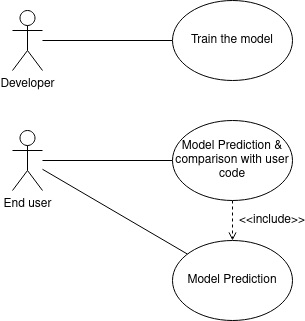
\includegraphics{use-case.drawio.png}    
    \caption{Діаграма прецедентів}
    \label{fig:use-case}
  \end{figure}

  \subsection{Внутрішнє проєктування}
  В додатку можна виділити наступні основні частини:
  \begin{itemize}[labelindent=\dimexpr\parindent*2\relax, leftmargin=*]
    \item інтерфейс користувача --- цей модуль буде перетворювати вхідні дані користувача на внутрішнє представлення та перевіряти коректність наданих даних. Також цей модуль відповідає за надання результату користувачу
    \item бекенд
      \begin{itemize}[labelindent=\dimexpr\parindent\relax, leftmargin=*]
        \item тренування моделі --- цей модуль буде додавати нові ключові слова до класів, знайдених у наданому тексті
        \item отримання припущення від моделі --- цей модуль буде надавати можливі класи до наданого тексту
        \item порівняння списків класів УДК --- цей модуль буде порівнювати два списки класів УДК, та надавати ступінь їх відповідності
      \end{itemize}
  \end{itemize}
  
  Також можна виділити такі типи даних (замість передавання рядка або числа між внутрішніми процедурами, зручніше передавати спеціалізовану структуру):
  \begin{itemize}[labelindent=\dimexpr\parindent*2\relax, leftmargin=*]
    \item Наукова робота/текст
    \item клас УДК
  \end{itemize}

  \subsection{Проєктування архітектури системи}
  Програму розроблено ітераціями. На кожну з ітерацій виділено окрему секцію. Є два типи ітерацій:
  \begin{enumerate}[labelindent=\dimexpr\parindent*2\relax, leftmargin=*]
    \item Реалізація нового функціоналу,
    \item Вдосконалення старого функціоналу.
  \end{enumerate}
  \subsubsection{Інтерфейс користувача}
  Для простоти тестування було вирішено почати розробку з інтерфейсу користувача.
  З попередніх секцій знаємо що це буде інтерфейс командного рядка.

  Найпростішим варіантом
  є перевірка аргументів командного рядка у функції main,
  і після цього виклик із цими аргументами внутрішньої реалізації.

  UML-діаграма для такої моделі виглядає наступним чином
  (Рис. \ref{fig:io_uml1}).
  Справжня реалізація буде мати складніший інтерфейс,
  але ця секція фокусуєтся на розробці користувацького інтерфейсу,
  тому на цьому єтапі реалізація представлена як дуже простий клас.

  \begin{figure}[H]
    \centering
    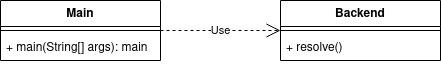
\includegraphics{io_uml1.drawio.png}    
    \caption{UML-діаграма 1}
    \label{fig:io_uml1}
  \end{figure}

  Алє таке рішення не є оптимальним ---
  заради простоти початкової реалізації
  втрачаєтся легкість подальшої заміні інтерфейсу.
  Тому доцільно виділити модуль який буде відповідати
  за взаємодію з користувачем.
  В нашому випадку це буде зчитування аргументів командного рядку,
  але за потреби він може бути замінений на графічний або веб-інтерфейс, тощо.
  Тепер діаграма виглядає так (Рис. \ref{fig:io_uml2}).

  \begin{figure}[H]
    \centering
    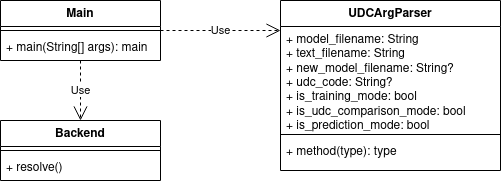
\includegraphics{io_uml2.drawio.png}    
    \caption{UML-діаграма 2}
    \label{fig:io_uml2}
  \end{figure}

  Тепер перед тим як викликати внутрішню реалізацію,
  main викликає клас UDCArgParser,
  який у свою чергу опрацьовує аргументи командного рядку.
  
  Хоча ця реалізація вирішує проблему відповідальності, вона додає декілька нових:
  \begin{itemize}[labelindent=\dimexpr\parindent*2\relax, leftmargin=*]
    \item по-перше UDCArgParser зчитує аргументи комадного рядка
    у конструкторі із глобальних змінних,
    це порушує принцип Dependency Inversion\cite{DI_wiki, SOLID_wiki};
    \item по-друге змінні is\_training\_mode, is\_udc\_comparison\_mode та \\ is\_prediction\_mode є взаємовиключними.
  \end{itemize}

  Для вирішення другої проблеми, потрібно скористатися поліморфізмом
  \cite{Polymorphism_wiki, Subtyping_wiki, Dynamic_dispatch_wiki}
  і замінити ці три змінні на одну,
  яка буде приймати значення одного з трьох підкласів.
  Іншими словами, треба заміни три взаємовиключні булеві змінні
  на одну змінну типу перечислення.
  З цими змінами UML-діаграма виглядає наступним чином (Рис. \ref{fig:io_uml3}).

  \begin{figure}[H]
    \centering
    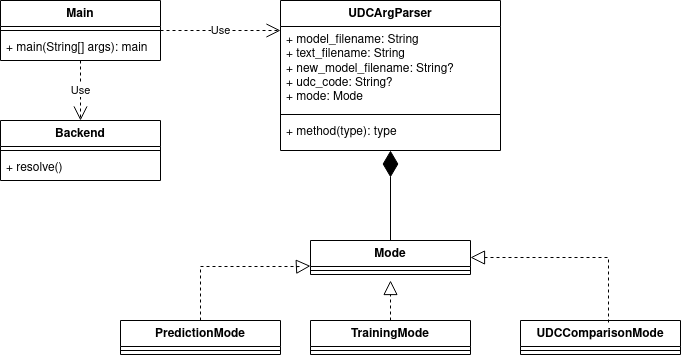
\includegraphics[width=\textwidth]{io_uml3.drawio.png}    
    \caption{UML-діаграма 3}
    \label{fig:io_uml3}
  \end{figure}
  
  Тепер клас Mode та його підкласи відповідають за представлення режиму,
  алє клас UDCArgParser має змінні new\_model\_filename та udc\_code,
  які в залежності від значення Mode завжди будуть NULL,
  тому доцільно перенести усі значення до підкласів Mode,
  перетворюючи тим самим це перечислення на алгебраічний тип данних
  \cite{ADT_wiki}.
  
  Доцільно помітити що алгебраічні типи даних відсутні в ООП та мові Python,
  тому вони будуть ємульовані з допомогою наслідування
  \cite{Code_complete_34_4, ADT_composition_over_inheritance}.
  
  Таким чином UDCArgParser дійсно буде мати тільки одну відповідальність ---
  перетворення аргументів командного рядка на об'єкт Mode.
  А Mode у свою чергу відповідає за представлення даних,
  які будуть надані внутрішній реалізації.
  Після цих змін UML-діаграма буде виглядати так (Рис. \ref{fig:io_uml4}).

  \begin{figure}[H]
    \centering
    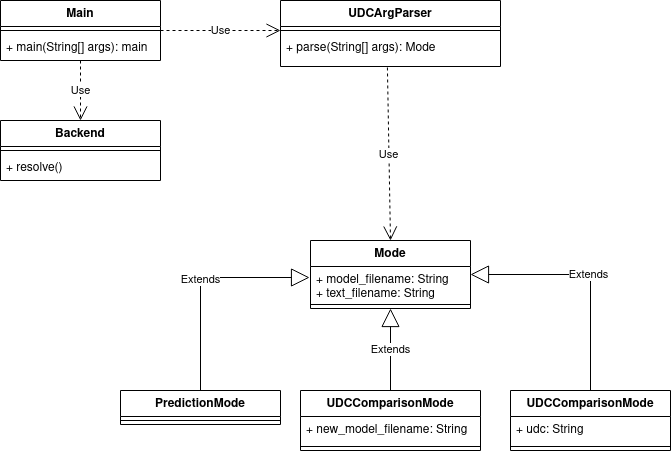
\includegraphics[width=\textwidth]{io_uml4.drawio.png}    
    \caption{UML-діаграма 4}
    \label{fig:io_uml4}
  \end{figure}
  
  Нова версія набагато краще попередніх, особливо першої.
  Втім все ще є недоліки:
  \begin{itemize}[labelindent=\dimexpr\parindent*2\relax, leftmargin=*]
    \item тип Mode містить поля model\_filename та text\_filename
    --- вони будуть передані в Backend
    (це не показано на діаграмах, тому теж є недоліком).
    Внутрішній реалізації потрібен вміст цих файлів,
    насправді внутрішня реалізація навіть не повинна знати що це вміст файлів,
    а не, наприклад, вміст текстового поля у графічному інтерфейсі, тощо.
    Тому доцільно:
      \begin{enumerate}[labelindent=\dimexpr\parindent\relax, leftmargin=*]
        \item Прибрати слово filename з обох полів,
        \item Виділити типи для цих значень ---
        таким чином ми зможемо робити майбутні зміни лише в одному місці
        % TODO: code complete ref (central control points or smth)
      \end{enumerate}
    \item Також присутня змінна new\_model\_filename в UDCComparisonMode ---
    вона так само не є важливою дла внутрішньої реалізації,
    а тільки для інтерфейсу користувача.
    Через те що для внутрішньої реалізації це буде одним з результатів
    (також можуть бути припущення щодо класів УДК та точності припущення,
    зробленного користувачем),
    це потрібно формалізувати в інтерфейсі класу Backend.
    \item Крім того, з попереднього пункту видно
    що потрібно формалізувати тип результату виконання внутрішньої реалізації.
    Втім, через те що маєтся чітка відовідність між підкласами Mode
    та типом (типами) результата внутрішньої реалізації доцільно розділити
    ці дії (режими роботи додатку) на окремі методи в класах Main та Backend.
  \end{itemize}

  \begin{figure}[H]
    \centering
    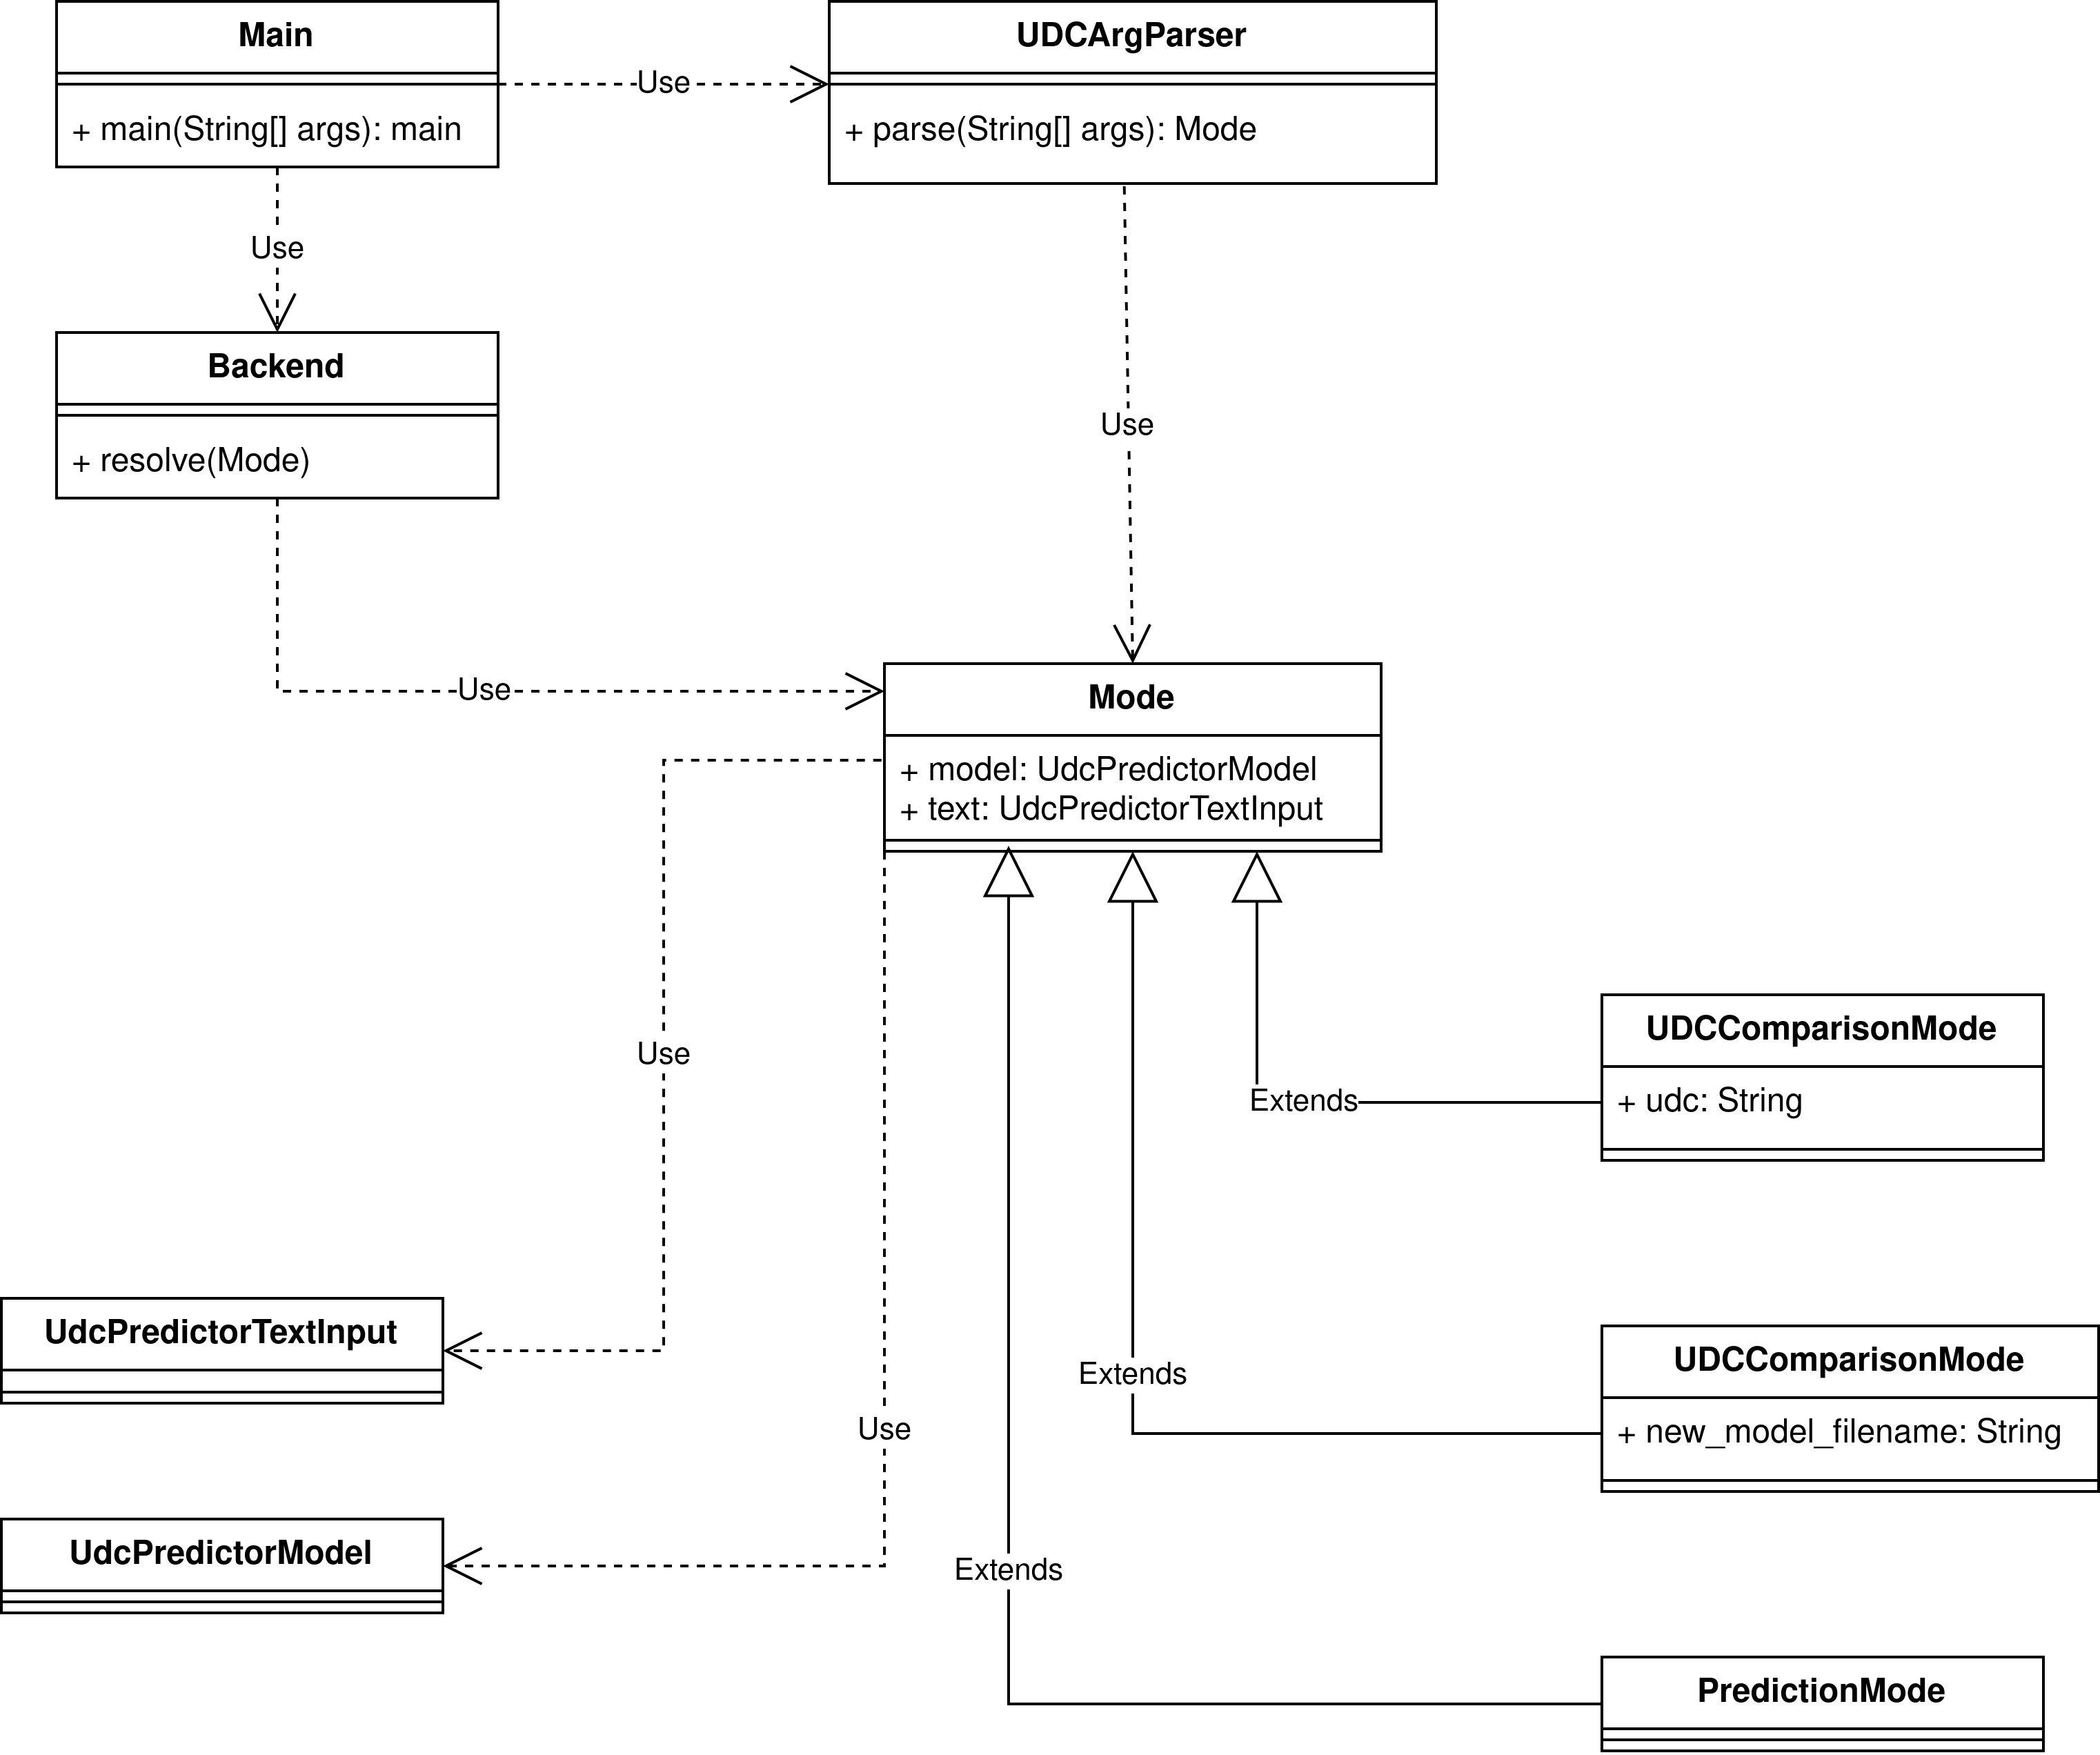
\includegraphics[angle=90, height=\textwidth]{io_uml5.drawio.png}    
    \caption{UML-діаграма 5}
    \label{fig:io_uml5}
  \end{figure}

  \subsection{Вибір засобів програмування}
  Для реалізації даного ПЗ було обрано мову Python,
  як найпопулярнішу в даному напрямі.
  Для вирішення задачі отримання ключових слів для заданого тексту
  потрібен такий функціонал:
  \begin{itemize}[labelindent=\dimexpr\parindent*2\relax, leftmargin=*]
    \item токенізація
    \item видалення стоп слів
    \item розмічування частин мови
    \item розпізнавання іменованих сутностей
  \end{itemize}
  або готовий алгоритм виділення ключових слів.
  Знайдено такі бібліотеки зі схожим функціоналом:
  \begin{itemize}[labelindent=\dimexpr\parindent*2\relax, leftmargin=*]
    \item RAKE (Rapid Automatic Keyword Extraction)
    \item YAKE (Yet Another Keyword Extractor)
    \item SpaCy
    \item NLTK (Natural Language Toolkit)
    \item TextBlob
    \item Gensim
  \end{itemize}

  YAKE потребує тренування на конкретному наборі даних ---
  не підходить для цього випадку з тієї самої причини що й класифікація.

  TextBlob є високорівневою обгорткою над NLTK,
  тому їх доцільно розглядати разом.
  Це бібліотеки загального призначення,
  але їх можна відкинути з наступних причин:
  \begin{itemize}[labelindent=\dimexpr\parindent*2\relax, leftmargin=*]
    \item вони програють SpaCy за швидкістю
    \item SpaCy має кращі моделі
    \item SpaCy має більш просунуті функції
  \end{itemize}

  Хоча SpaCy не має готового алгоритму витягування ключових слів,
  його дуже легко реалізувати.

  Алгоритм, який використовує RAKE працює наступним чином ---
  текст розбивається на слова, потім перевіряється частота слів,
  та ступінь їх появи з іншими,
  слова сортуються за обома критеріями з попереднього кроку.

  SpaCy не надає готово алгоритму виділення ключових слів,
  але дає можливість розбити текст на слова, розмічати їх як частини мови,
  розпізнати іменовані сутності.

  Алгоритм RAKE чисто статистичний і має більшу похибку ---
  він може вважати за ключові слова такі,
  які не є вагомими та навпаки виключати важливі.

  Gensim не має деяких важливих алгоритмів
  для реалізації витягування ключових слів,
  а ті які є в цій бібліотеці були розроблені, в першу чергу,
  для інших цілей і не є оптимальними для нашої задачі.
  З цього виходить що SpaCy є найкращим вибором:
  \begin{itemize}[labelindent=\dimexpr\parindent*2\relax, leftmargin=*]
    \item має весь потрібний функціонал
    \item має моделі
    \item швидше за інші бібліотеки
  \end{itemize}

  \subsection{Перетворення ключових слів на класи УДК}
  В наведених у попередніх розділах відкритих каталогах УДК
  кількість ключових слів для кожного з підкласів дуже мала
  (близько 10 на кожен підклас), тому буде згенеровано свій каталог.
  Алгоритм створення наступний:
  \begin{enumerate}[labelindent=\dimexpr\parindent*2\relax, leftmargin=*]
    \item Беремо ключові слова з існуючої роботи (ті які надав автор),
    \item Витягуємо ключові слова з тексту з допомогою обраного алгоритму,
    \item Порівнюємо ключові слова з п.1 та п.2 та додаємо до каталогу ті,
    які входять до обох списків.
  \end{enumerate}

  Точність такого підходу буде напряму залежати від кількості розглянутих робіт
  та кількості отриманих ключових слів.
  Через обмежений час такі каталоги будуть створені не для усіх підкласів,
  та деякі класи будуть мати меншу вибірку.

  \subsection{Висновки}

  \section{РОЗРОБКА ПРОГРАМИ}
  \subsection{Розробка інтерфейсу користувача}
  Для простоти виконання буде використано інтерфейс командного рядка (CLI). 
  Для цієї задачі в мові python є спеціалізований модуль argparse.

  З розробленої use-case діаграми можна сказати шо є два режими роботи
  (стільки  ж скільки й акторів).
  Через те що режими тільки два, доцільно використати прапор.
  Основним сценарієм є припущення,
  тому прапор буде використовуватися для тренування "\-\-training".
  
  Модель та текст присутні на вході кожного випадку,
  тому їх можна зробити позиційними аргументами.
  
  Список класів є тільки в одному випадку,
  тому це буде опціональним аргументом,
  який буде прийматися тільки якщо відсутній прапор "\-\-training",
  цей аргумент буде помічатись як "\-\-udc".
  Для припущення результат буде надаватися в stdout у наступному форматі:
  список класів та ступінь їх відповідності, якщо використано "\-\-udc".
  
  Маємо такі сценарії використання:
  \begin{enumerate}
    \item Тренування моделі
      \begin{mycode}[caption={Тренування моделі}, label={code:training_ex}]
        $ udc-classifier \
            model.model \
            scientific-work.txt \
            --training updated-model.model
      \end{mycode}
      \begin{itemize}
        \item udc-classifier --- назва виконуваного файлу
        \item model.model --- назва файлу існуючої моделі
        \item scientific-work.txt --- назва файлу з текстом наукової роботи
        \item updated-model.model --- назва файлу, до якого буде записано нову модель
      \end{itemize}
    
    \item Отримання припущення
      \begin{mycode}[caption={Отримання припущення}, label={code:result_prompt_ex}]
        $ udc-classifier model.model scientific-work.txt
      \end{mycode}
      \begin{mycode}[caption={Припущення (класи, які можуть підійти до наданого тексту)}
                    , label={code:result_ex}]
        539.120 94 084.3
      \end{mycode}
      \begin{itemize}
        \item udc-classifier --- назва виконуваного файлу
        \item model.model --- назва файлу існуючої моделі
        \item scientific-work.txt --- назва файлу з текстом наукової роботи
      \end{itemize}

    \item Отримання припущення та порівняння класів
      \begin{mycode}[caption={Отримання припущення та порівняння класів}, label={code:result_prompt_ex2}]
        $ udc-classifier \
            model.model \
            scientific-work.txt \
            --udc ‘913(574.22)"19"(084.3)’
      \end{mycode}
      \begin{mycode}[caption={Припущення}
                    , label={code:result_ex2}]
        539.120 94 084.3
        0.3
      \end{mycode}
      \begin{itemize}
        \item udc-classifier --- назва виконуваного файлу
        \item model.model --- назва файлу існуючої моделі
        \item scientific-work.txt --- назва файлу з текстом наукової роботи
        \item третій рядок прикладу ---
        класи, які можуть підійти до наданого тексту
        \item другий рядок --- вхідний шифр УДК
        \item четвертий рядок --- ступінь відповідності класів
        (від 0 до 1, де 0 --- відсутні співпадіння, 1 --- повне співпадіння)
      \end{itemize}
  \end{enumerate}


  \subsection{Висновки}

  \section{ТЕСТУВАННЯ ТА НАЛАГОДЖЕННЯ}
  \subsection{Висновки}
  \BgThispage

  \unnumberedSection{ЗАГАЛЬНІ ВИСНОВКИ ТА РЕКОМЕНДАЦІЇ}
  \BgThispage

  \phantomsection
  \printbibliography[heading=bibintoc, title=СПИСОК ВИКОРИСТАНОЇ ЛІТЕРАТУРИ]

  \unnumberedSection{ДОДАТКИ}
  \BgThispage

\end{document}
